{\color{indiagreen}\subsection{Standard Assets}}
To je velika skupina assetov, ki je spravljena v en paket. Unity je naredil ta paket, da lahko začetniki hitro in brez večjega truda naredijo enostavno aplikacijo. V tem paketu je tudi veliko primerov uporabe teh assetov. Zelo olajšajo kakšne stvari, za katere bi enemu samemu razvijalcu vzelo veliko časa, da bi jih implementiral. V mojem projektu sem tudi uporabila Joystick implementacijo iz standard assetov. To sem naredil tako, da sem šel \textbf{Assets} $\rightarrow$ \textbf{Import Package} in izbral področje katerega sem želel (v mojem primeru je to bilo CrossPlatformInput).\\
\begin{figure}[ht!]
	\centering
	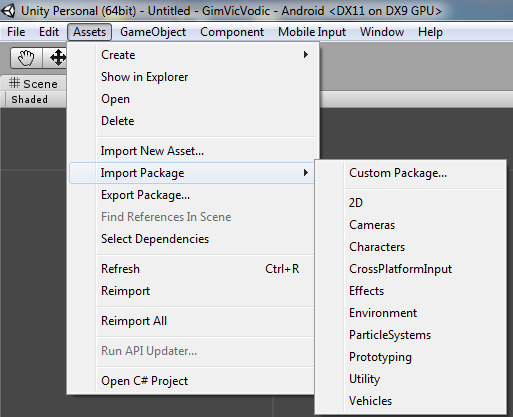
\includegraphics[width=8cm, height=8cm,keepaspectratio=true]{Importing7.png}
	\caption{Standard Assets}
\end{figure}
In nato se odpre okno, ki ga lahko vidimo tudi na sliki 9.\\
Je pa tudi velika past saj z vsako novo verzijo Unity-ja pridejo novo standard asseti, ki se lahko obnašajo drugače, kot prejšnji zato moramo vedno pogledati za kakšno verzijo, so bili izdani asseti.